\section{Experimental Results}

%\paragraph{Task/Problem.}
As many real-world datasets contain missing values, missing data imputation (MDI) has been a popular problem to tackle in statistics and machine learning~\cite{little1986statistical, nelwamondo2007missing}.
GNNs have recently proved to be a powerful tool for this task~\cite{spinelli2020neural}.
With a view that our method incorporates additional higher-dimensional structure in the data, we evaluate the performance of the SNNs in imputing missing data over simplicial complexes.

\paragraph{Data.}
A \emph{co-authorship complex}~\cite{patania2017} is a simplicial complex where a paper with $k$ authors is represented by a $(k-1)$-simplex.
\mdeff{Projection of the paper-author bipartite graph? Discuss why not hypergraphs? Not sure.}\stefania{I think it is important to point out this general setting. I added an explanation in the appendix. If we'll have still space, I'll move it here.}
By subset closure, vertices represent authors and the added subsimplices of the $k-1$-simplex are interpreted as collaborations among subgroups of authors. We sampled two co-authorship complexes---CC1 and CC2, see Table~\ref{table:Simplices-coauthor} for statistics---from the Semantic Scholar Open Research Corpus~\cite{ammar18NAACL}, a dataset of over $39$ million research papers with authors and citations.\footnote{Papers with less than $5$ citations and more than $10$ authors were excluded.}
\mdeff{I have a repo with the code to create this dataset. Shall we make it public and link it here?}\stefania{Sure!}
We believe the following procedure extracts representative papers from which one can construct co-authorship complexes: We performed random walks (of length $80$) on the vertices of the graph which correspond to papers, and edges connect papers sharing at least one author. \mdeff{Needs clarification.}\stefania{You think it is not clear why we do the random walks?or how?}
The $k$-cochains are given by the number of shared citations of the given collaboration (see Figure~\ref{fig:data2complex} and~\ref{fig:bipartite}).
\mdeff{Could be more precise. Though the figure is great and very helpful.}\stefania{I added something in the appendix together with a figure. What do you think? In a longer version this will be definitely clarified here.}

\paragraph{Method.}
We evaluated the performance of the SNNs on the task of imputing missing data on the $k$-cochains (for $k=0,1,2$) of the extracted co-authorship complexes. As in a typical pipeline for this task~\cite{nelwamondo2007missing}, missing data is artificially introduced by replacing a portion of the values with a constant. Specifically, given a fixed co-authorship complex, missing data is introduced at random on the $k$-cochains at $4$ rates: $10\%,  20\%,  30\%$, and $50\%$. The training input is then given by the $k$-cochains on which the random missing data is substituted by the median of the known data (the median is perhaps a reasonable first guess for estimating missing data). We trained an SNN comprising $3$ layers with $30$ convolutional filters of degree $N=5$. We used the $L_1$ norm as the reconstruction loss over the known elements, and the Adam optimizer with a learning rate of $10^{-3}$. The SNN was trained for $1000$ iterations. We then tested the performance of the network on its accuracy in imputing missing data. As a statistical evaluation, we tested the network on different random samples of the damaged portions for the same percentage of missing value.

\paragraph{Results.}
\gard{Note for me to remember to add a punchline somewhere in this section :-)}
Figure~\ref{fig:accuracy-error} (a-b) shows the mean accuracy (MA) and mean absolute error distribution (MAED) \stefania{change we do not take average histogram} (see Section~\ref{sec:supp_material} for definitions) of the SNN in inputing missing citations on CC1. Observe that the distribution of the prediction error accumulates close to zero.

%\begin{figure}[htbp]
%  \centering
%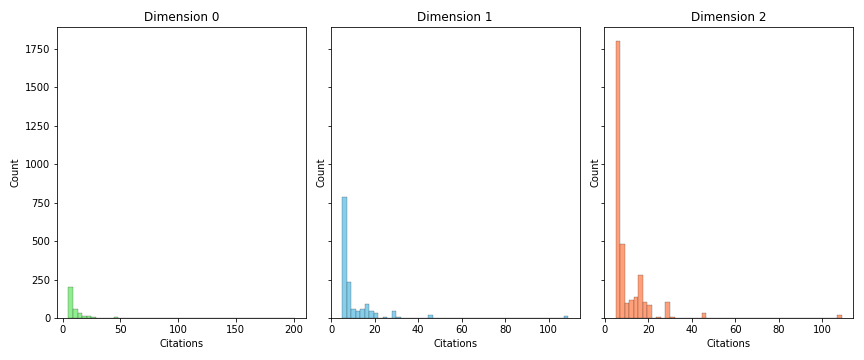
\includegraphics[scale=0.35]{./figures/distribution_cohain_150250.png}
% \caption{Distribution of the citation in CC1 } \label{fig:accuracy}
%\end{figure}
\begin{figure}[tb]
\centering
 \begin{subfigure}[t]{-0.8\textwidth}
 \vspace{-4cm}
    \text{(a)}
  \end{subfigure}
\begin{subfigure}[t]{0.8\textwidth}
\centering
   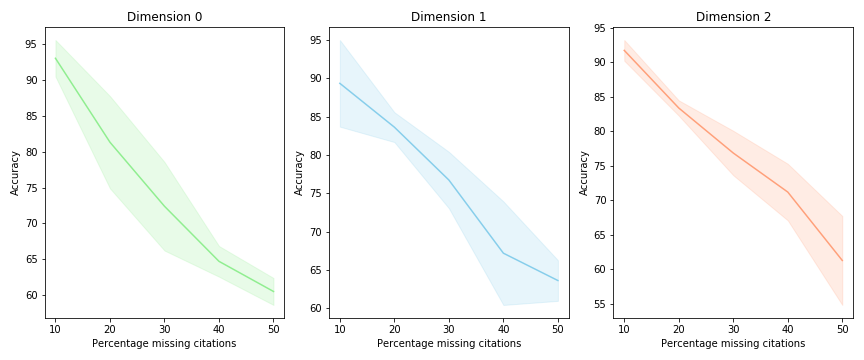
\includegraphics[scale=0.35]{./figures/accuracy_network1.png}
 %\caption{Accuracy of SNN in predicting missing citations } \label{fig:accuracy}
\end{subfigure}
 \begin{subfigure}[t]{0.8\textwidth}
    \text{(b)}
  \end{subfigure}
\begin{subfigure}[t]{0.8\textwidth}
\centering
\vspace{-0.5cm}
   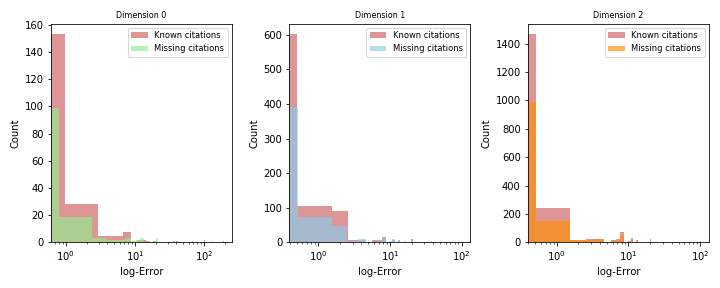
\includegraphics[scale=0.36]{./figures/Error_dist_start150250_seed6666_notsee40.png}
 % \caption{Distribution of the prediction's error} \label{fig:error}
\end{subfigure}
\caption{(a) Mean Accuracy $\pm$ std over 5 samples of SNN in imputing missing citations on CC1. (b) Mean Absolute Error $\pm$ std over 5 samples of SNN for $40\%$ missing values in CC1. \stefania{Add error on bins.} \mdeff{I don't get (b).} \mdeff{Some space could be claimed from this figure.}}
\label{fig:accuracy-error}
\end{figure}

As a second assessment, we evaluate how accurately an SNN trained on one co-authorship complex can impute missing citations on a different complex. Over the assumption that co-authorship complexes share a similar structure and the same data underlies the generating process of cochains.
Figure~\ref{fig:transfer-learning} shows the MA in predicting missing citations on CC1 using the above architecture of SNN trained on CC2.
\mdeff{Conclusion? Trained SNN transfer because not much MA is lost, or the hypothesis is satisfied?}\stefania{I think the SNN transfer because of the similarity of the complexes (and therefore Laplacians), I can write down this as an hypothesis but it needs to be further investigated (ie are the kernels of the laplacians similar?are the homologies of the complexes the same?..)}

Table~\ref{table:comparison-SNN} shows the performance of three statistical baselines: missing values inferred as the mean or median of all known values, and missing values inferred from the $(k-1)$ and $(k+1)$ neighbors of the simplices ($k$-simplicial neighbor $k$-sn).
\mdeff{Mean or median of the neighbors?}
SNNs well outperform these baselines.
Comparison with other state-of-the-art imputation algorithms is left for future work.

\begin{figure}[htbp]
  \centering
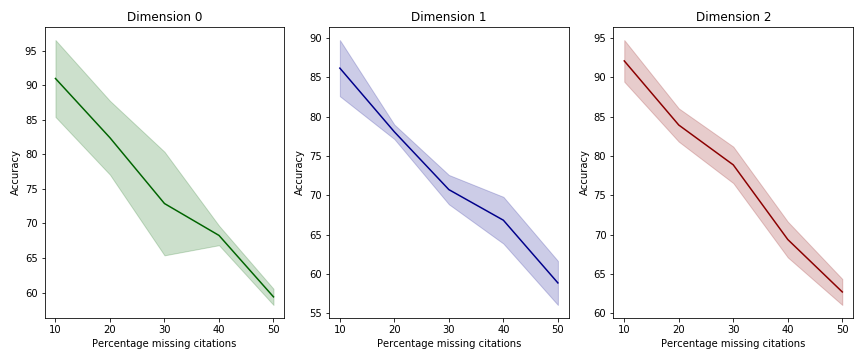
\includegraphics[scale=0.35]{./figures/accuracy_network1_pretrained.png}
  \caption{Mean Accuracy $\pm$ std over 5 samples in imputing missing citations on CC1 with an SNN trained on CC2.} \label{fig:transfer-learning}
\end{figure}

%\scriptsize{
\begin{table}[htbp]
  \centering
  \scriptsize{
  \begin{tabular}{lcccccc}
    \toprule
    Method   & CC1 - dim 0   & CC1 - dim 1   & CC1 - dim 2   & CC2 - dim 0  & CC2 - dim 1  & CC2 - dim 2 \\
    \midrule
    Global Mean & $3.3 \pm 0.82$ & $5.75\pm 1.28$  &$ 2.96\pm 0.49$  & $3.32 \pm 0.85$ & $8.31 \pm 1.03$  & $7.90\pm 0.35$\\
    Global Median & $7.78 \pm 0.7$   & $10.44 \pm 1.$ &$ 12.75 \pm 0.63 $ & $5.76 \pm 0.38 $&$ 6.3\pm 0.36  $&$ 6.11\pm 0.2$\\
    $k$-sn & $30.89\pm 5.47 $& $33.97 \pm 1.92$ & $39.43 \pm 0.83  $& $21.67 \pm 2.67 $&$ 29.26\pm 1.35$   &$ 32.36 \pm 0.5 $\\
    \bottomrule
  \end{tabular}}
   \vspace{2pt}
  \caption{%
      Performance of statistical baselines: Mean Accuracy $\pm$ standard deviation for $30\%$ of missing data over 5 samples. \stefania{Add uniform distribution sampling instead of mean?}
 \mdeff{Align on period and $\pm$.}
  }\label{table:comparison-SNN}
\end{table}%}
